\chapter{Badania symulacyjne}\label{chap:research}


% \section{Porównanie wyników optymalizacji z literaturą~\cite{evolutionary_puredata}}

Praca wykorzystuje próbki dźwięku z literatury~\cite{evolutionary_puredata_results}
aby przetestować zaimplementowany algorytm i jednocześnie porównać jego wyniki
z podobną pracą. Wykorzystano te próbki dźwięku
z literatury, które \textbf{nie zostały wygenerowane} za pomocą
oprogramowania do syntezy \textit{Pure Data}~\cite{pure_data},
ponieważ oryginalna praca wykorzystywała
to oprogramowanie jako środowisko do syntezy dźwięku -- takie porównanie
nie byłoby miarodajne, ponieważ algorytm z literatury miałby do dyspozycji
dokładnie takie same algorytmy, które zostały wykorzystane do wygenerowania
dźwięków docelowych.
Przed przeprowadzeniem optymalizacji ustalono wartość częstotliwości podstawowej~$f_0$
dla każdego z testowanych dźwięków, aby algorytm optymalizował parametry kontrolujące
jedynie barwę dźwięku dla z góry zadanej właściwej wysokości dźwięku.
Podobną praktykę stosują badania z literatury~\cite{ieee_synth_programming}.
Zastosowano implementację algorytmu estymującego częstotliwość podstawową
\textit{YIN}~\cite{yin_pitch_estimation}, dostępną w pakiecie obliczeniowym
\texttt{librosa}~\cite{librosa}. Przebieg procesu optymalizacji dla każdego z testowanych
dźwięków umieszczony jest na płycie CD, co opisuje dodatek~\ref{chap:opis-plyty}.

\subsubsection{Parametry algorytmu genetycznego}

W badaniach zastosowano następujące parametry algorytmu genetycznego:

\begin{enumerate}
  \item rozmiar populacji: \texttt{50},
  \item liczba iteracji: \texttt{200},
  \item strategia mutacji: \texttt{best1bin},
  \item rekombinacja: \texttt{0.7}.
\end{enumerate}

Ze względu na długi czas działania zaimplementowanego algorytmu optymalizacji
(średnio 10 minut na pojedynczą iterację),
w pracy nie udało się porównać jak różne parametry algorytmu genetycznego
wpływają na proces optymalizacji. Finalnie wykonano tylko jedną pełną optymalizację
dla każdego z testowanych dźwięków.

\newpage

\section{Dźwięk fletu}

Dźwięk \texttt{flute.wav}~(rysunek~\ref{fig:literature_flute_sound_overview})
jest nagraniem prawdziwego instrumentu dętego. Kształt fali jest nieregularny,
charakterystyka spektralna zawiera dynamicznie pojawiające się i słabnące 
składowe częstotliwościowe.

% \begin{multicols}{3}
\begin{figure}[H]
    \centering
    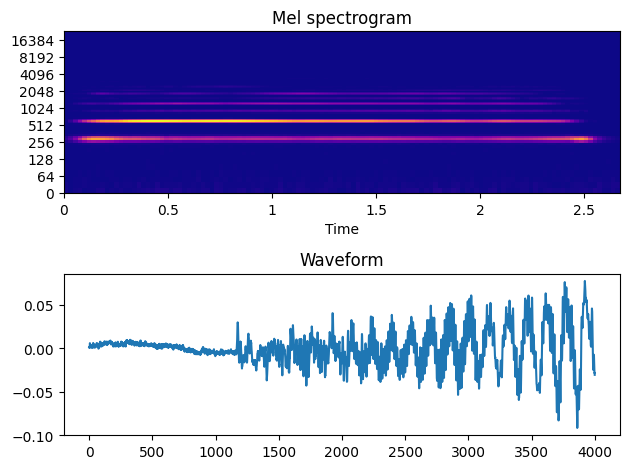
\includegraphics[width=0.7\linewidth]{rys06/target_sample_flute_literature.png}
    \caption{
      Spektrogram i wykres fali dla dźwięku \texttt{flute.wav} wykorzystywanego
      do eksperymentów w~\cite{evolutionary_puredata_results}.
    }\label{fig:literature_flute_sound_overview}
\end{figure}

\begin{figure}[H]
    \centering
    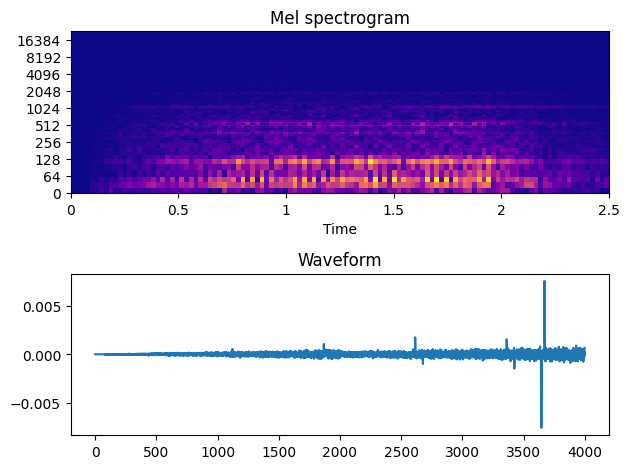
\includegraphics[width=0.7\linewidth]{rys06/evolved_sample_flute.png}
    \caption{
      Spektrogram i wykres fali dla dźwięku \texttt{flute.wav}
      wytworzonego przez zaimplementowany algorytm optymalizacji
      dla dźwięku \texttt{flute.wav}.
    }\label{fig:evolved_flute_sound_overview}
\end{figure}

\begin{figure}[H]
    \centering
    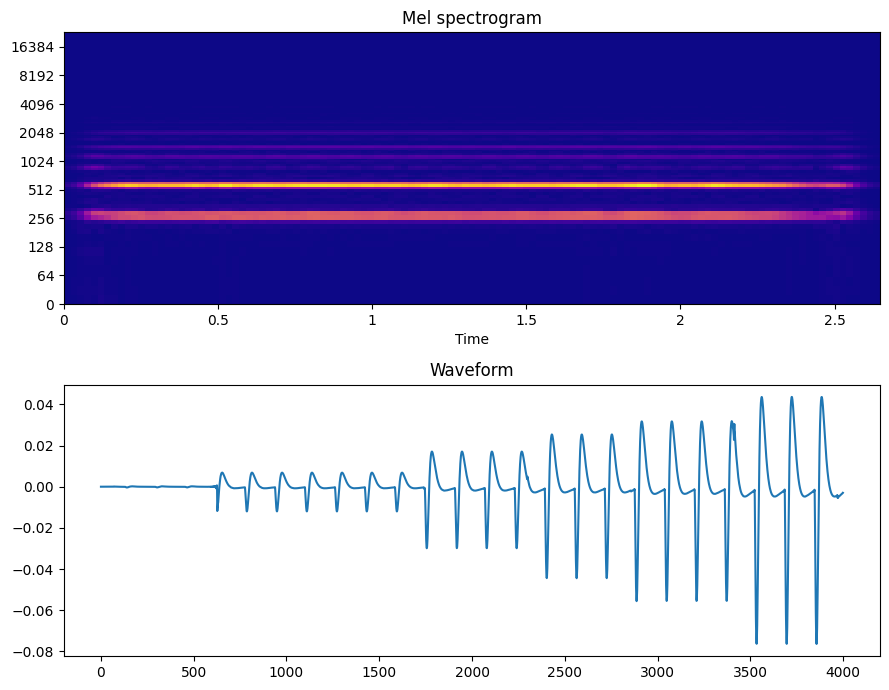
\includegraphics[width=0.7\linewidth]{rys06/macret_evolved_flute.png}
    \caption{
      Spektrogram i wykres fali dla dźwięku
      wygenerowanego przez algorym z literatury~\cite{evolutionary_puredata}
      na wzór \texttt{flute.wav}.
    }\label{fig:evolved_literature_flute}
\end{figure}
% \end{multicols}

\begin{figure}[H]
    \centering
    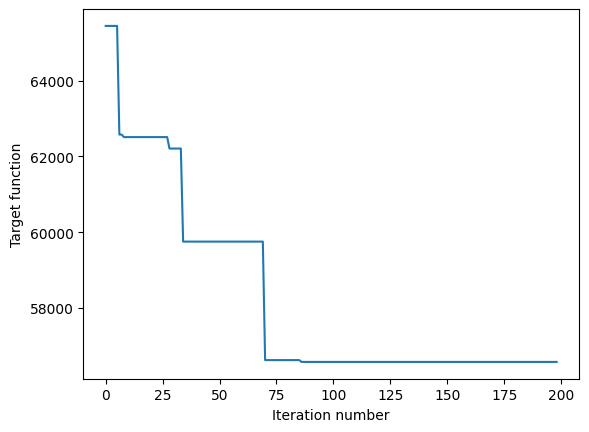
\includegraphics[width=0.6\linewidth]{rys06/flute_target_fun_values.png}
    \caption{
      Zmiany wartości funkcji celu podczas optymalizacji.
    }%\label{fig:evolved_literature_flute}
\end{figure}


Zaimplementowany algorytm nie jest w stanie przybliżyć dźwięku fletu.
Wygenerowany sygnał przedstawiony na rysunku~\ref{fig:evolved_flute_sound_overview}
zawiera nieregularne częstotliwości składowe,
jednak nie pokrywają się one z częstotliwościami w dźwięku docelowym.
Wygenerowane składowe o niskiej częstotliwości zupełnie nie występują w dźwięku docelowym.
Na wygenerowanej strukturze grafu (rysunek~\ref{fig:evolved_graph_flute}) widoczny
jest filtr wysokoprzepustowy (\texttt{HighPassFilter \#11}), co pozwala wnioskować,
że odfiltrowanie niskich częstotliwości poprawiało uzyskiwane wartości funkcji celu.

\begin{figure}[H]
    \centering
    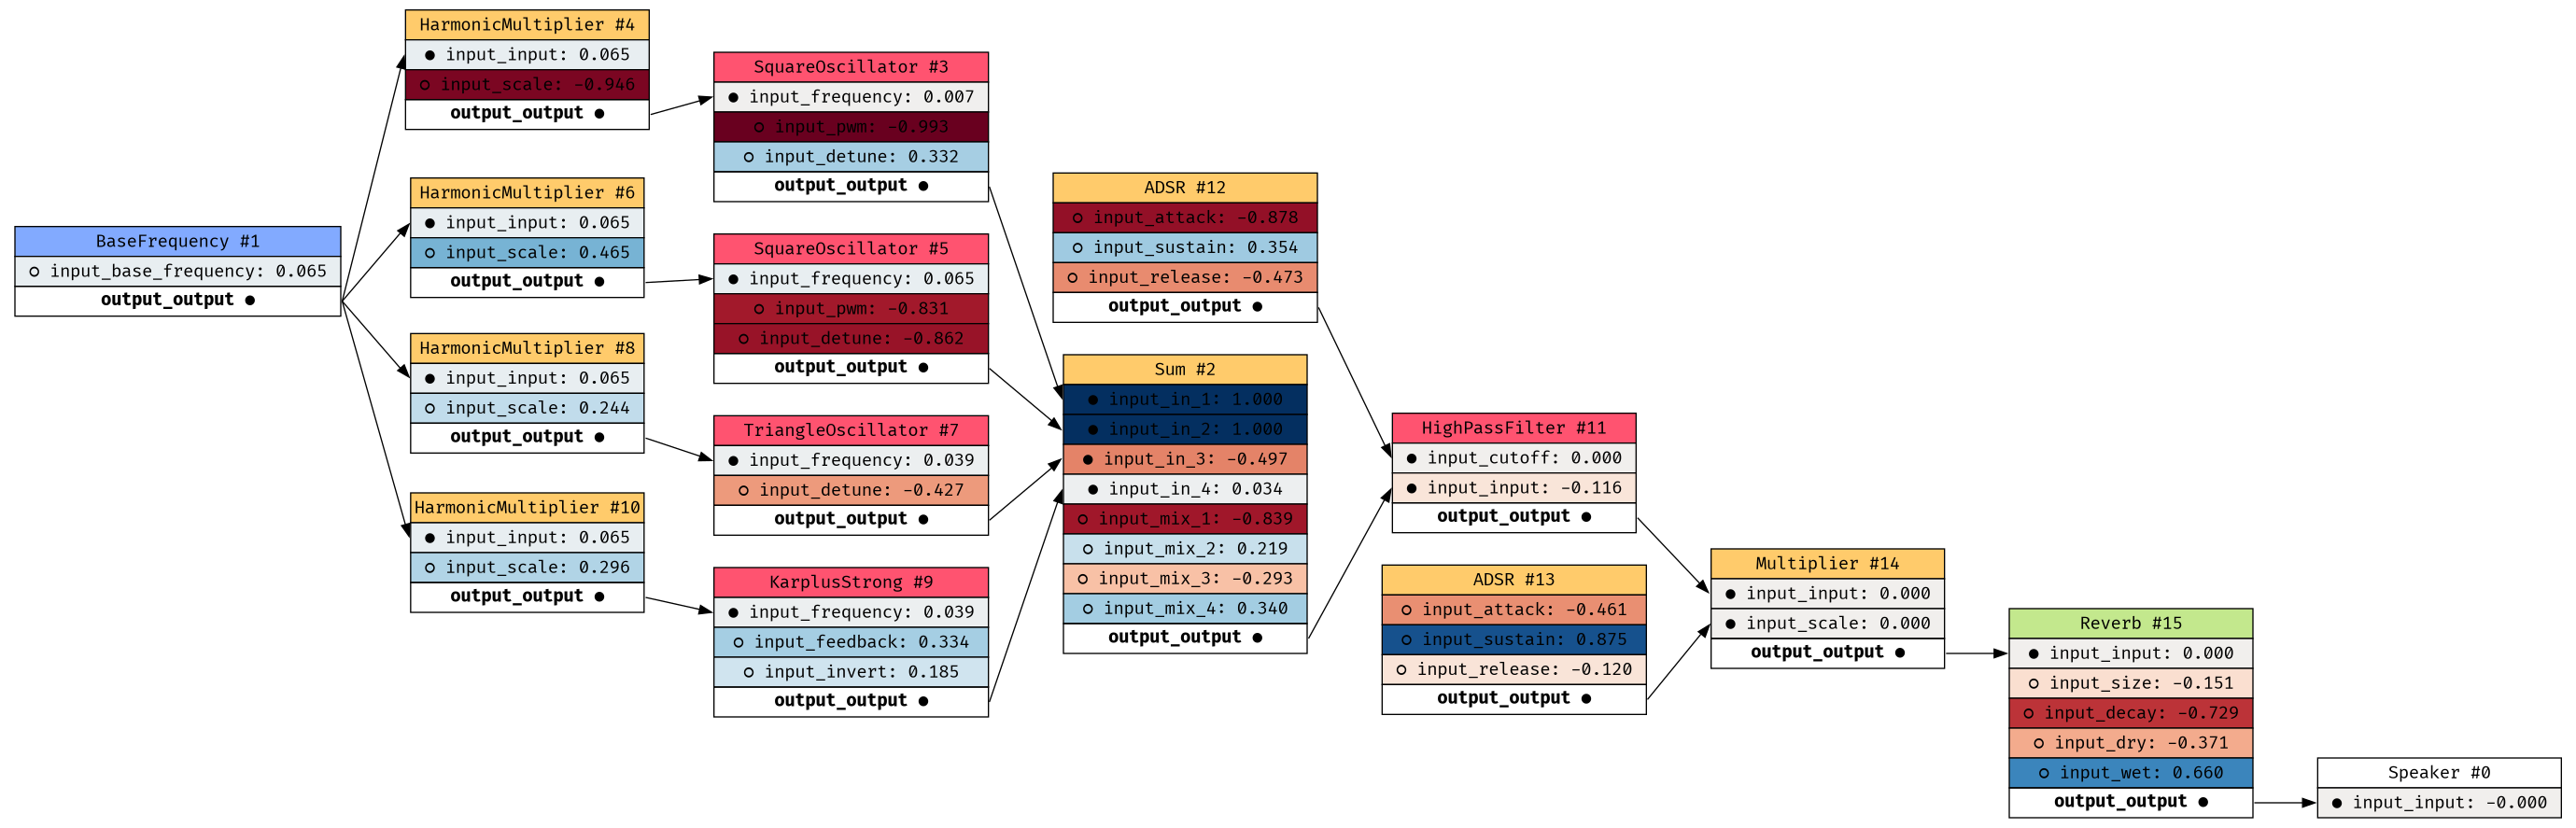
\includegraphics[angle=90,width=0.45\linewidth]{rys06/evolved_graph_flute.png}
    \caption{
      Graf DSP wygenerowany przez zaimplementowany algorytm
      dla dźwięku docelowego \texttt{flute.wav}.
    }\label{fig:evolved_graph_flute}
\end{figure}



\section{Sampel z syntezatora \textit{OP-1}}

Dźwięk \texttt{op1\_1.wav}, wygenerowany przy pomocy syntezatora \textit{OP-1} jest próbą
zasymulowania dźwięku instrumentu dętego przez syntezator. Podobnie jak w przypadku
prawdziwego dźwięku fletu, widoczne są zmienne w czasie składowe harmoniczne, jednak
sygnał wygenerowany na syntezatorze jest bardziej stabilny.

% \begin{multicols}{3}
\begin{figure}[H]
    \centering
    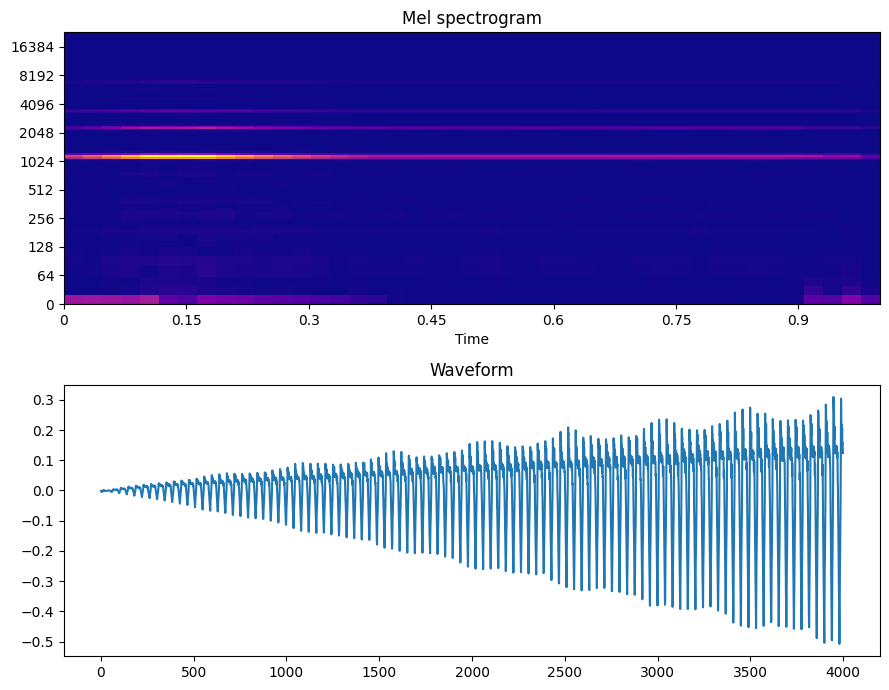
\includegraphics[width=0.7\linewidth]{rys06/target_sample_op1_literature.png}
    \caption{
      Spektrogram i wykres fali dla dźwięku \texttt{op1\_1.wav} wykorzystywanego
      do eksperymentów w~\cite{evolutionary_puredata_results}.
    }\label{fig:literature_op_1_sound_overview}
\end{figure}


\begin{figure}[H]
    \centering
    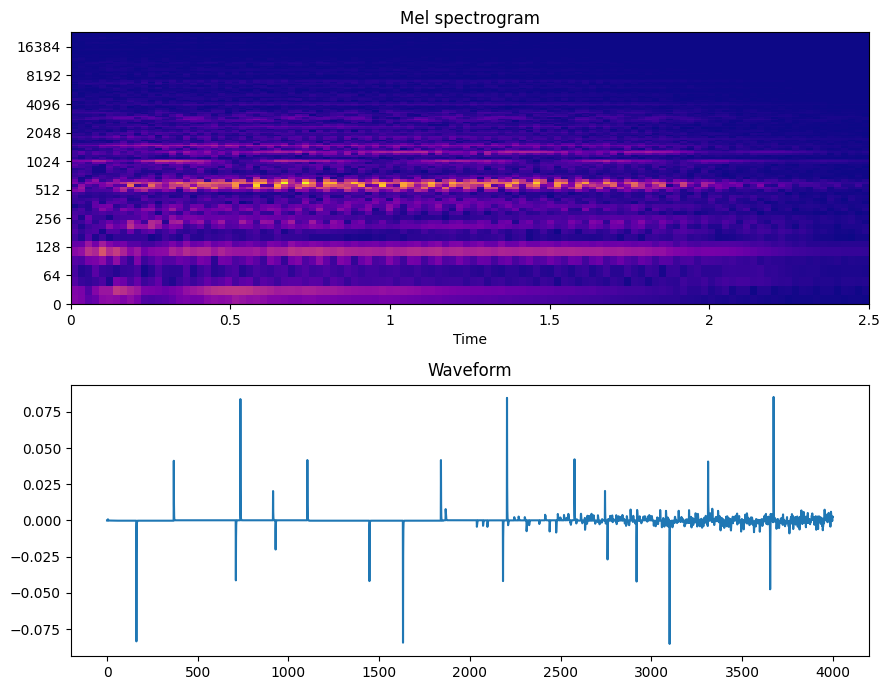
\includegraphics[width=0.7\linewidth]{rys06/evolved_sample_op1.png}
    \caption{
      Spektrogram i wykres fali dla dźwięku wygenerowanego
      przez algorytm optymalizacji na wzór \texttt{op1\_1.wav}.
    }\label{fig:evolved_op1_sound_overview}
\end{figure}


\begin{figure}[H]
    \centering
    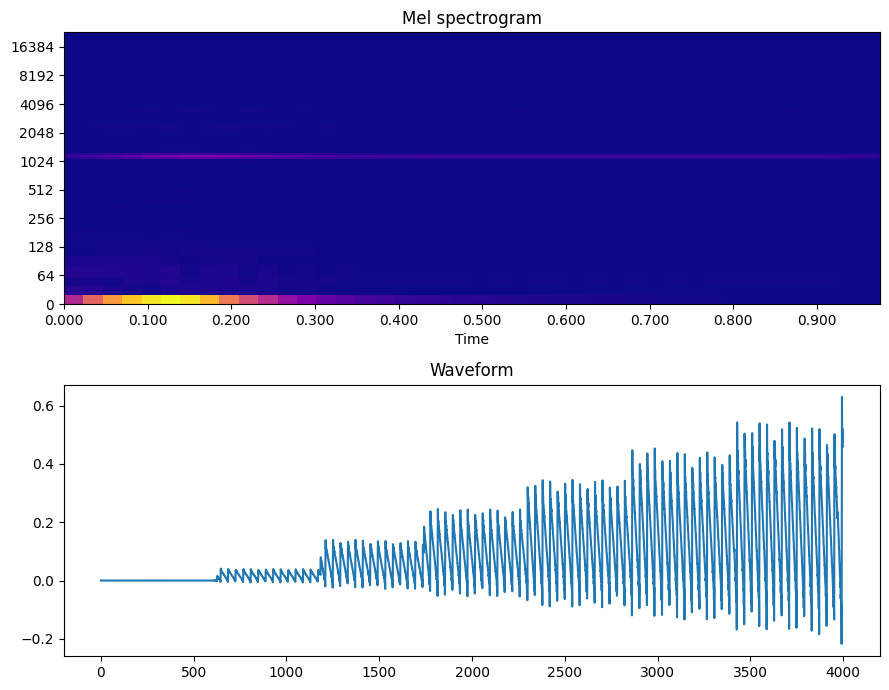
\includegraphics[width=0.7\linewidth]{rys06/macret_evolved_op1.png}
    \caption{
      Spektrogram i wykres fali dla dźwięku wygenerowanego
      przez algorytm z literatury~\cite{evolutionary_puredata} na wzór \texttt{op1\_1.wav}.
    }\label{fig:evolved_literature_op1_sound_overview}
\end{figure}
% \end{multicols}

\begin{figure}[H]
    \centering
    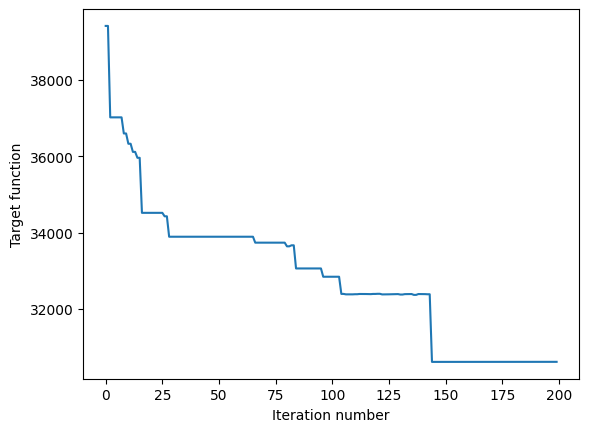
\includegraphics[width=0.6\linewidth]{rys06/op1_target_fun_values.png}
    \caption{
      Zmiany wartości funkcji celu podczas optymalizacji.
    }%\label{fig:evolved_literature_flute}
\end{figure}

Zaimplementowany algorytm generuje dźwięk bliski do szumu, wygenerowane
składowe częstotliwościowe nie pokrywają się z dźwiękiem docelowym.
Algorytm z literatury lepiej przybliża docelowy dźwięk -- odtwarza
pojedynczą częstotliwość składową, widoczną na rysunku~\ref{fig:literature_op_1_sound_overview}.

\begin{figure}[H]
    \centering
    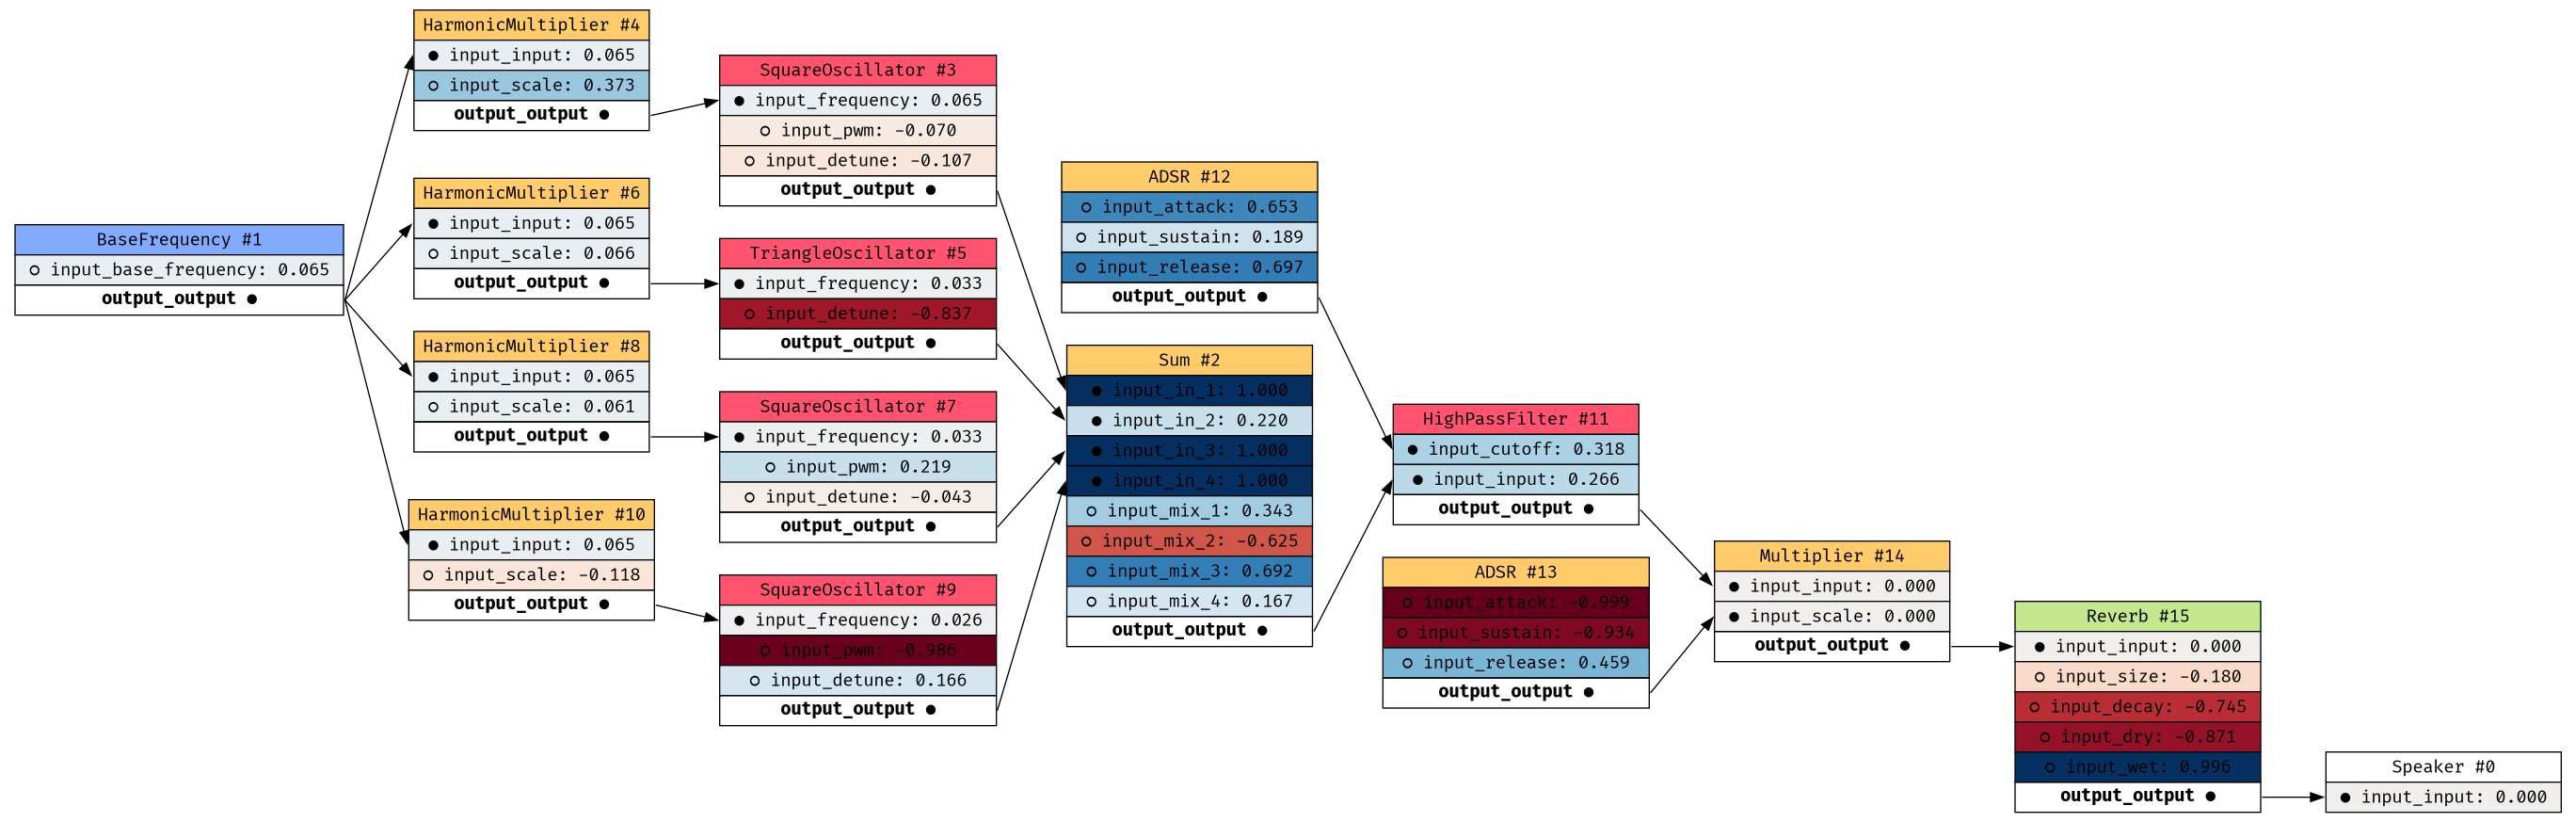
\includegraphics[angle=90,width=0.45\linewidth]{rys06/evolved_graph_op1.png}
    \caption{
      Graf DSP wygenerowany przez zaimplementowany algorytm
      dla dźwięku docelowego \texttt{op1\_1.wav}.
    }\label{fig:evolved_literature_op1_sound_overview}
\end{figure}

\section{Transjent}

Dźwięk \texttt{transient.wav}, przedstawiony na rysunku~\ref{fig:literature_transient_sound_overview},
został wykorzystany w literaturze~\cite{evolutionary_puredata} do sprawdzenia jak dobrze algorytm
generujący dźwięk potrafi przybliżyć dźwięki o dynamicznych zmianach w charakterystyce spektralnej.
Tego typu dźwięki przypominają brzmienie instrumentów klawiszowych: fortepianu lub klawesynu.

% \begin{multicols}{3}
\begin{figure}[H]
    \centering
    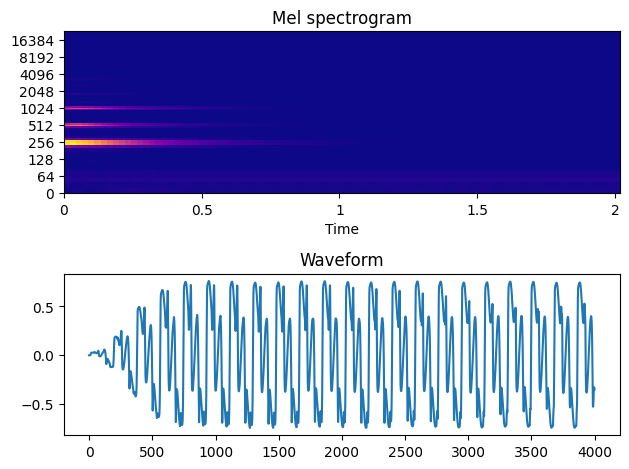
\includegraphics[width=0.7\linewidth]{rys06/transient_sample_literature.png}
    \caption{
      Spektrogram i wykres fali dla dźwięku \texttt{transient.wav} wykorzystywanego
      do eksperymentów w~\cite{evolutionary_puredata_results}.
    }\label{fig:literature_transient_sound_overview}
\end{figure}

\begin{figure}[H]
    \centering
    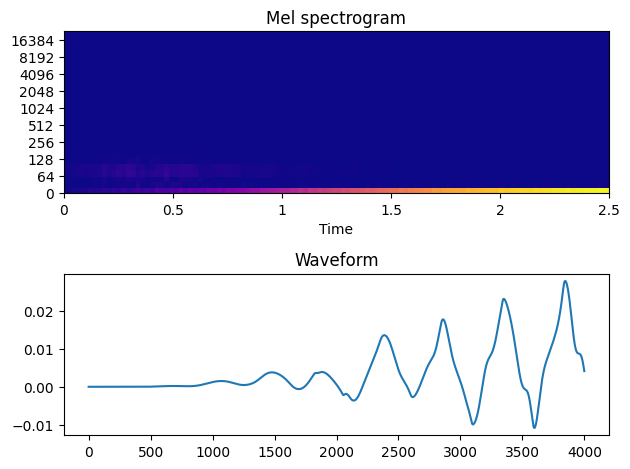
\includegraphics[width=0.7\linewidth]{rys06/evolved_sample_transient.png}
    \caption{
      Spektrogram i wykres fali dla dźwięku wygenerowanego na wzór
      \texttt{transient.wav}.
    }\label{fig:evolved_transient_sound_overview}.
\end{figure}

\begin{figure}[H]
    \centering
    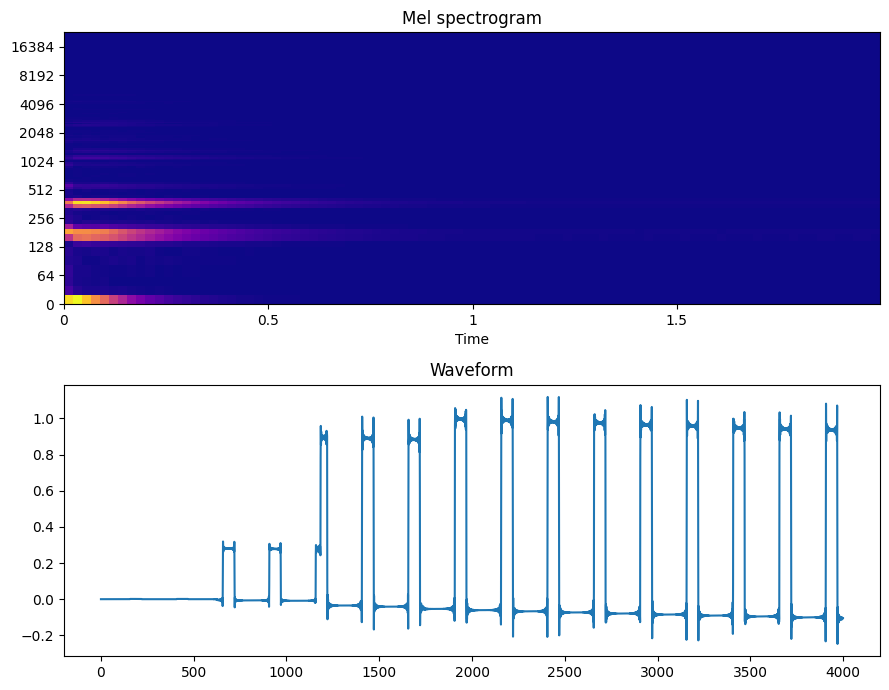
\includegraphics[width=0.7\linewidth]{rys06/macret_evolved_transient.png}
    \caption{
      Spektrogram i wykres fali dla dźwięku wygenerowanego 
      przez algorytm z literatury~\cite{evolutionary_puredata} na wzór
      \texttt{transient.wav}.
    }\label{fig:evolved_literature_transient_sound_overview}.
\end{figure}
% \end{multicols}

\begin{figure}[H]
    \centering
    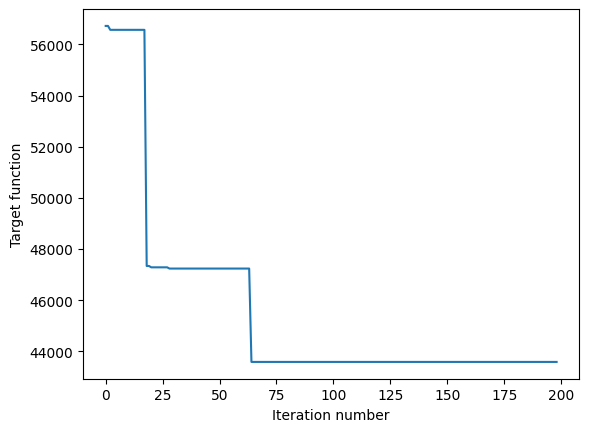
\includegraphics[width=0.6\linewidth]{rys06/transient_target_fun_values.png}
    \caption{
      Zmiany wartości funkcji celu podczas optymalizacji.
    }%\label{fig:evolved_literature_flute}
\end{figure}

\begin{figure}
    \centering
    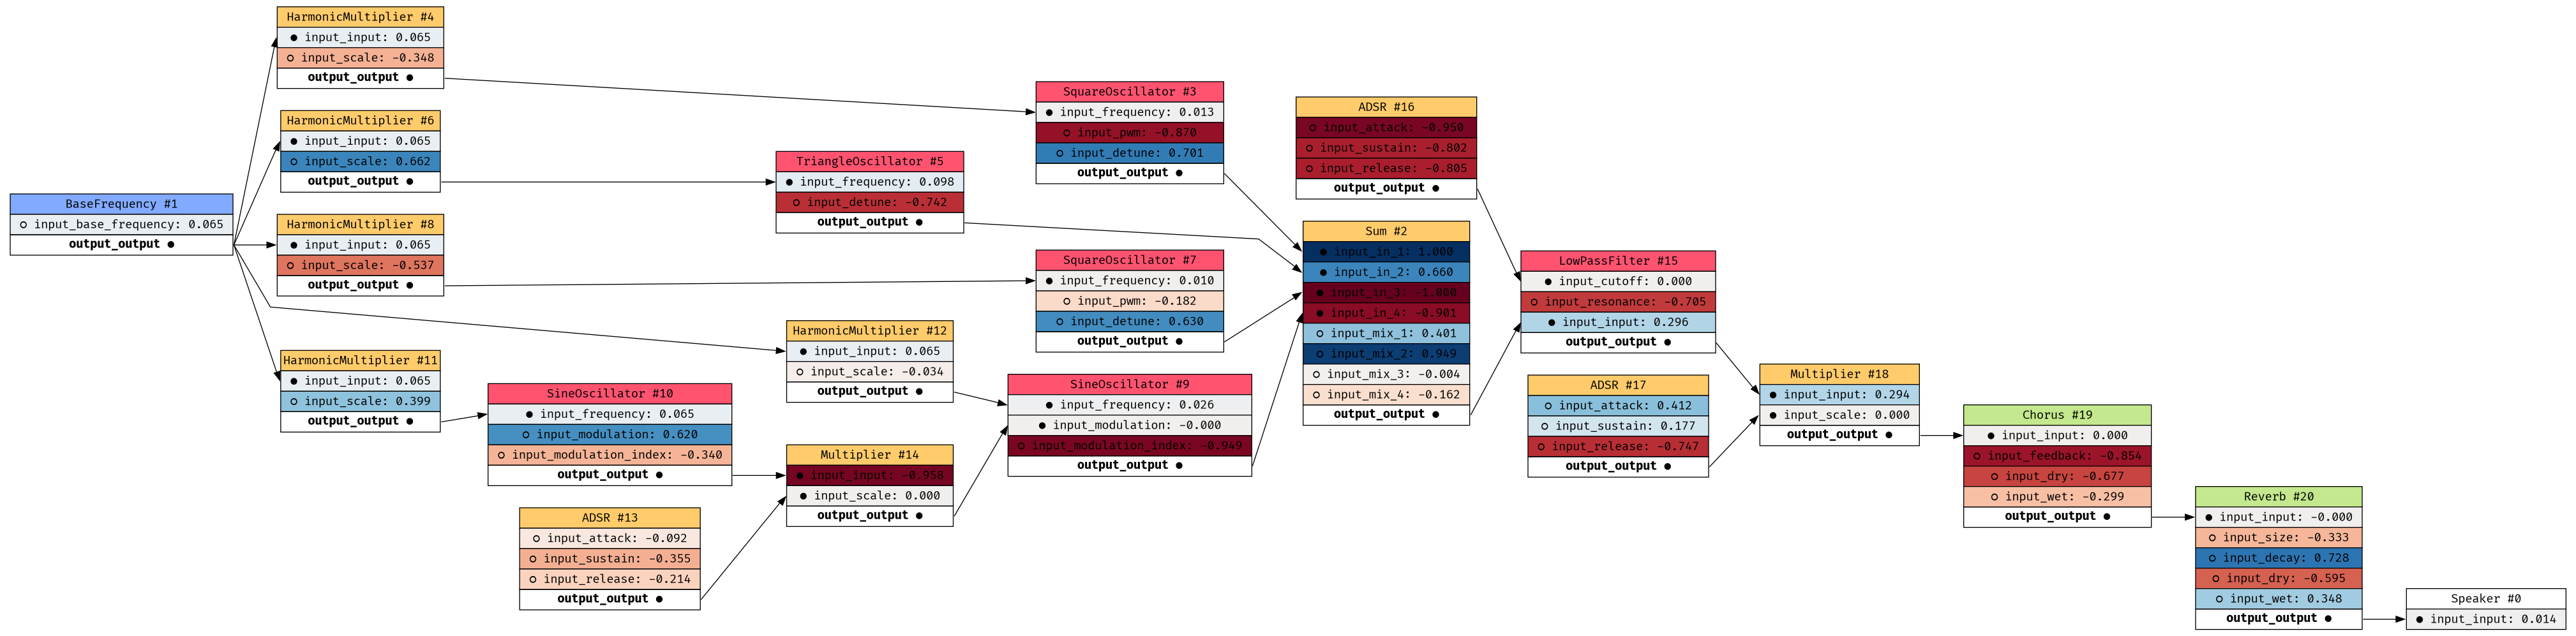
\includegraphics[angle=90,width=0.35\linewidth]{rys06/evolved_graph_transient.png}
    \caption{
      Graf DSP wygenerowany przez zaimplementowany algorytm
      dla dźwięku docelowego \texttt{transient.wav}.
    }\label{fig:evolved_graph_transient}
\end{figure}



\section{Dźwięki inne niż przykłady z literatury}\label{sec:non_literature_samples}

Badania przeprowadzone w ramach~\cite{evolutionary_puredata}
wykorzystują ograniczony zbiór dźwięków, koncentrując
się na instrumentach dętych i syntezie FM\@. Algorytm przetestowano
również na samodzielnie wytworzonych dźwiękach, wykorzystując syntezę
subtraktywną~\ref{fig:minilogue_target_sample}.

% \begin{multicols}{2}
\begin{figure}[H]
    \centering
    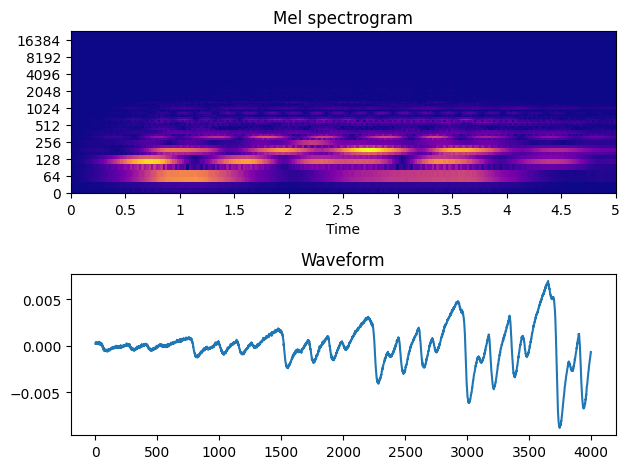
\includegraphics[width=0.7\linewidth]{rys06/target_minilogue.png}
    \caption{
      Spektrogram i wykres fali dla dźwięku wygenerowanego 
      na syntezatorze \textit{Korg Minilogue xd}.
    }\label{fig:minilogue_target_sample}
\end{figure}

\begin{figure}[H]
    \centering
    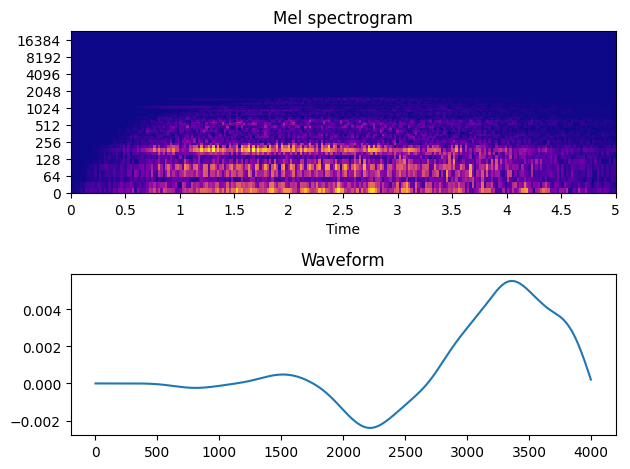
\includegraphics[width=0.7\linewidth]{rys06/evolved_minilogue.png}
    \caption{
      Spektrogram i wykres fali dla dźwięku wygenerowanego 
      przez zaimplementowany w ramach pracy algorytm na
      wzór~\ref{fig:minilogue_target_sample}.
    }\label{fig:evolved_minilogue_sample}.
\end{figure}
% \end{multicols}


\begin{figure}
    \centering
    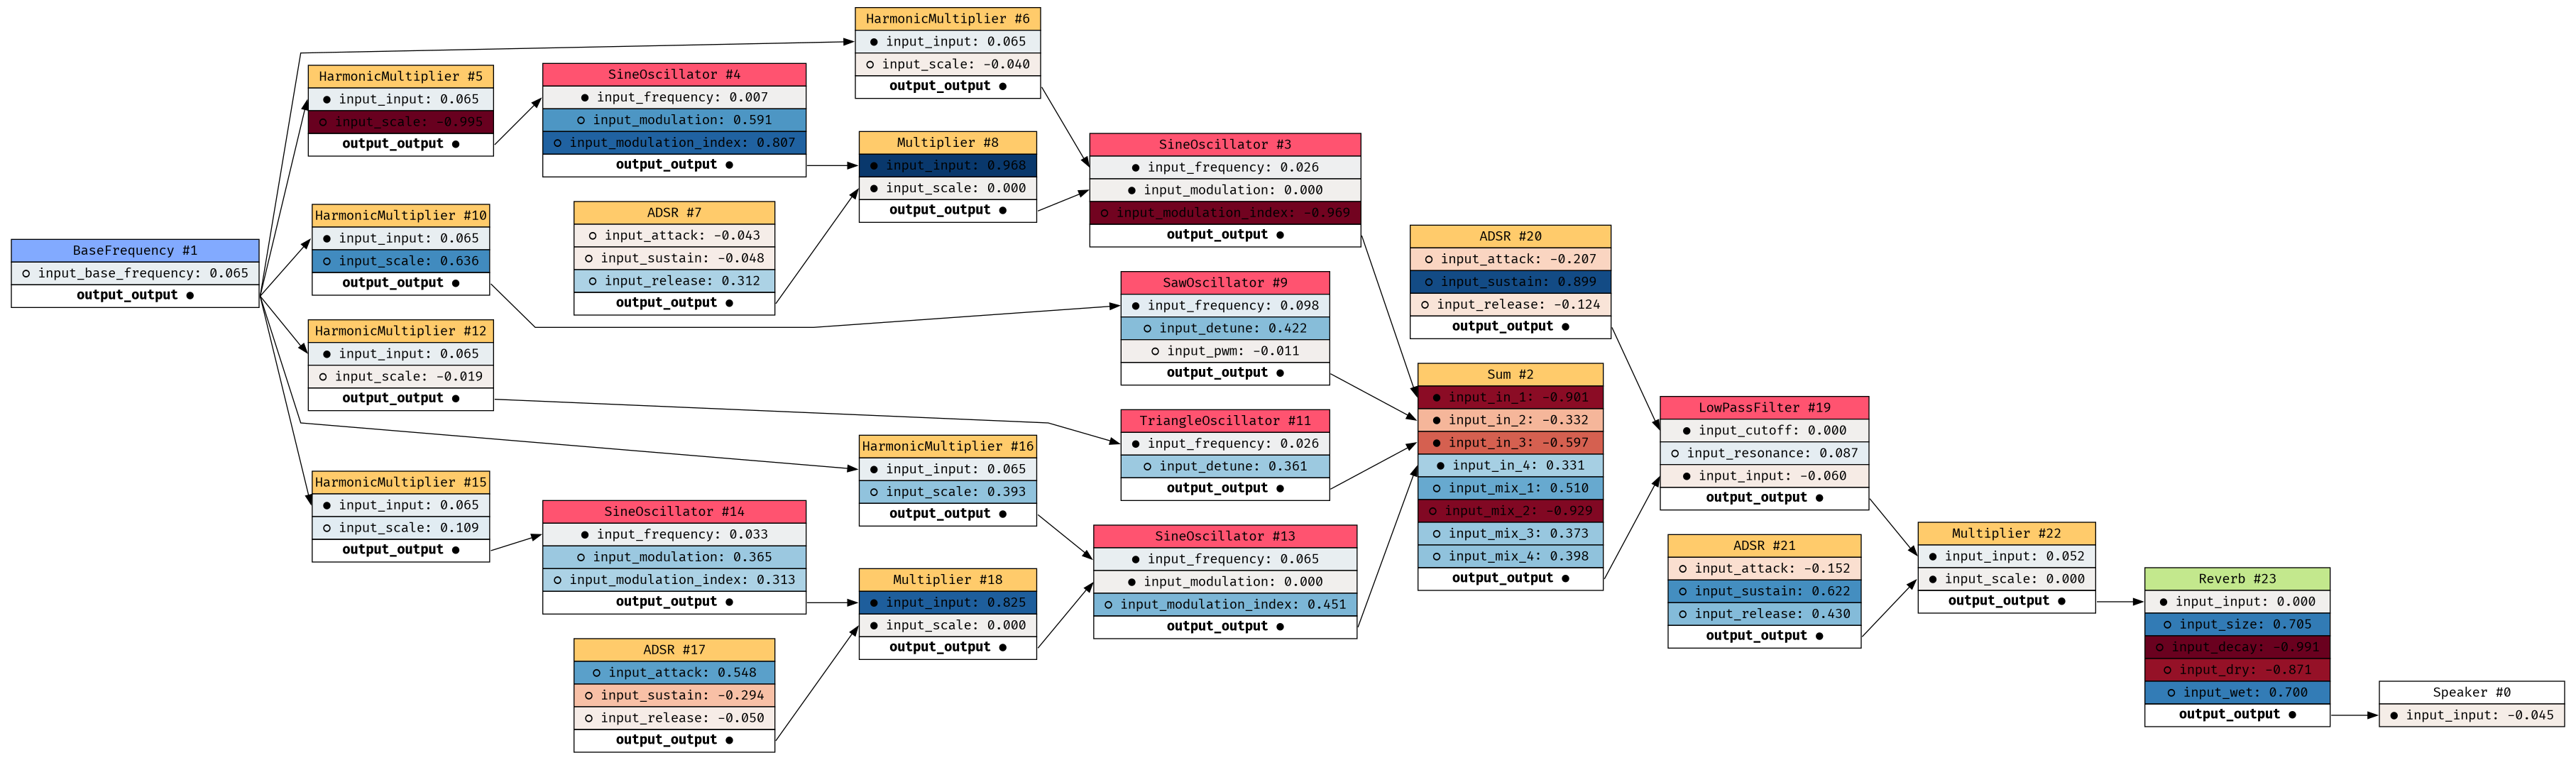
\includegraphics[angle=90,width=0.44\linewidth]{rys06/evolved_graph_minilogue.png}
    \caption{
      Graf DSP wygenerowany przez zaimplementowany algorytm
      dla dźwięku docelowego~\ref{fig:minilogue_target_sample}.
      Poprawnie został odtworzony filtr niskoprzepustowy oraz
      sterujący nim sygnał ADSR\@.
    }\label{fig:evolved_graph_op1}
\end{figure}

